% Introdução

\documentclass[Tese.tex]{subfiles}

\begin{document}
	
\chapter{Modelo termo-elástico}\label{ch:termo-elasticidade}

A partir deste capítulo, são tratados modelos com acoplamento termo-mecânico, isto é, onde os problemas térmico e mecânico atuam conjuntamente e de forma interdependente. Particularmente, é apresentado o modelo termo-elástico, no qual a parcela mecânica é considerada um sólido hiperelástico.

\section{Base termodinâmica}

No caso termo-elástico, a energia livre de Helmholtz $\helmholtz$ pode ser escrita apenas em função da deformação ($\E$) e da temperatura. Assim, sua taxa pode ser expressa como:
\begin{equation}
\dothelmholtz(\E,\temp) = \dfrac{\partial \helmholtz}{\partial \E}:\dotE + \dfrac{\partial \helmholtz}{\partial \temp}\dottemp.
\end{equation}
Aplicando essa equação nas leis da termodinâmica, \cref{eq:primeira-lei-2,eq:clausius-duhem}, resulta:
\begin{align}
& \left(\dfrac{\partial \helmholtz}{\partial \E} - \S\right):\dotE  + \left(\dfrac{\partial \helmholtz}{\partial \temp} +  {\entropy}\right)\dottemp  + \temp \dotentropy - \calorInt + \gradientei\cdot\qi = 0, \label{eq:primeira-lei-mod} \\
&\dissipation = \left(\S - \dfrac{\partial \helmholtz}{\partial \E}\right):\dotE - \left({\entropy} + \dfrac{\partial \helmholtz}{\partial \temp}\right)\dottemp - \dfrac{1}{T}\qi\cdot\gradientei\,\temp \geq 0. \label[ineq]{eq:clausius-duhem-mod}
\end{align}

Uma vez que $\dotE$ e $\dottemp$ são arbitrários, os termos entre parênteses devem ser igualados a zero para que as leis da termodinâmica sejam atendidas. Isso resulta nas seguintes relações constitutivas:
%\begin{equation}
\begin{equation}
\S = \dfrac{\partial \helmholtz}{\partial \E} \text{\qquad e\qquad} \entropy=-\dfrac{\partial \helmholtz}{\partial \temp}.\label{eq:const2} 
\end{equation}
Consequentemente, a \cref{eq:primeira-lei-mod} e a \cref{eq:clausius-duhem-mod} resultam nas seguintes expressões:
\begin{align}{ }
&
\temp \dotentropy - \calorInt + \gradientei\cdot\qi = 0, \label{eq:cond0}
\\[0.1cm]
&
\qi\cdot\gradientei\,\temp \leq 0. \label[ineq]{eq:cond-termo}
\end{align}
%\end{equation}
As Eqs. \eqref{eq:const2} são denominadas relações constitutivas do material. A primeira, já apresentada na \cref{eq:S}, é incorporada no problema mecânico, enquanto a segunda é incorporada no problema térmico. A partir da \cref{eq:const2}, obtém-se:
\begin{equation}\label{eq:dotentropy}
\dotentropy = -\dfrac{\partial^2 \helmholtz}{\partial \temp \partial\E}:\dotE - \dfrac{\partial^2 \helmholtz}{\partial \temp^2}\dottemp = \operadorTermoElastico:\dotE + \dfrac{\volumetricHeatCapacity}{\temp}\dottemp,
\end{equation}
onde $\volumetricHeatCapacity$ é o calor específico volumétrico, já definido na \cref{eq:specific-heat}, e $\operadorTermoElastico$ é denominado operador termo-elástico, dado por
\begin{equation}
\operadorTermoElastico = -\dfrac{\partial^2 \helmholtz}{\partial \temp \partial\E} = \dfrac{\partial\entropy}{\partial\E}.
\end{equation}

Aplicando-se a \cref{eq:dotentropy} na \cref{eq:cond0}, temos a equação local de condução de calor para o problema termo-elástico:
\begin{equation}\label{eq:equacao-conducao-local}
\gradientei\cdot\qi + \temp\operadorTermoElastico:\dotE + \volumetricHeatCapacity\dottemp = \calorInt.
\end{equation}
O termo $\temp\operadorTermoElastico:\dotE$ é denominado termo de acoplamento termo-elástico, responsável por transmitir o calor gerado pelas deformações elásticas ao problema térmico.

É conveniente expressar a energia livre de Helmholtz através da decomposição aditiva entre uma parcela mecânica ($\helmholtzm$), dependente da deformação e da temperatura, e uma parcela térmica ($\helmholtzt$), dependente apenas da temperatura, isto é:
\begin{equation}
\helmholtz(\E,\temp) = \helmholtzm(\E,\temp) + \helmholtzt(\temp).
\end{equation}
Para a parcela térmica, pode-se utilizar a lei dada por \citeonline{vujovsevic2002finite}, apresentada na \cref{eq:helmholtz-t-0}. Isto é:
\begin{equation}\label{eq:helmholtz-t}
\helmholtzt(\temp) = (\specificHeatIni-\specificHeatConst\tempref)\left(\temp-\tempref-\temp \ln{\dfrac{\temp}{\tempref}}\right)-\dfrac{1}{2}\specificHeatConst(\temp-\tempref)^2.
\end{equation}
Já a parcela mecânica pode ser expressa na forma $\helmholtzm(\E,\temp) = \helmholtzm(\Ee,\temp)$, onde $\Ee$ é a parcela puramente elástica da deformação, dependente da deformação total e da temperatura. Uma vez escrita nessa forma, $\helmholtzm$ pode ser dada por uma lei hiperelástica análoga às discutidas na \autoref{sec:hiper}. Resta, portanto, avaliar como será definido o tensor $\Ee$. Neste trabalho, duas formas serão discutidas: a decomposição aditiva e a multiplicativa.

\section{Decomposição aditiva}\label{eq:te-dec-aditiva}

Na termo-elasticidade linear, é comum assumir que a deformação linear de engenharia pode ser expressa pela soma entre parcelas elástica e térmica. Esse conceito pode ser generalizado considerando a decomposição aditiva do tensor de deformações de Green-Lagrange, isto é:
\begin{equation}\label{eq:dec-aditiva}
\E = \Ee + \Et
\end{equation}
onde $\Ee$ é a parcela elástica, e $\Et$ é a parcela térmica da deformação, definida pela lei de expansão térmica do material, que depende apenas da temperatura. Para o caso de pequenas deformações, muitos materiais podem ser representados pela seguinte lei linear\footnote{Embora seja utilizada nos desenvolvimentos algébricos desta subseção, essa lei linear apresentada não será de interesse nas aplicações numéricas deste trabalho, sendo substituída por outra lei na \autoref{sec:equivalencia-leis-expansao}.}:
\begin{equation}\label{eq:expansao-linear-0}
\Et = (\temp-\tempref)\boldsymbol{\coefExp},
\end{equation}
onde $\boldsymbol{\coefExp}$ é o tensor de coeficientes de expansão térmica. Levando-se em conta que $\Et$ representa puramente os efeitos de dilatação ou contração, apenas suas parcelas da diagonal principal devem ser não-nulas, isto é, $\coefExp_{ij}=0$ para $i \ne j$. Além disso, para o caso termicamente isotrópico, considerado neste trabalho, temos $\boldsymbol{\coefExp} = \coefExp\I$, onde $\coefExp$ é um coeficiente único de expansão térmica. Assim, a \cref{eq:expansao-linear-0} pode ser escrita como:
\begin{equation}\label{eq:expansao-linear}
\Et = \coefExp(\temp-\tempref)\I,
\end{equation}
de forma que
\begin{equation}\label{eq:Ee-expansao-linear}
\Ee = \E - \coefExp(\temp-\tempref)\I.
\end{equation}

Observa-se, no entanto, que a lei linear dada na \cref{eq:expansao-linear-0} deve ser aplicada somente ao caso de pequenas deformações, uma vez que ela não é limitada para valores excessivos de contração, o que pode provocar a inversão do material.

O modelo constitutivo mecânico pode ser definido em função de $\Ee$ conforme as leis hiperelásticas apresentadas na \autoref{sec:hiper}. Assim, calcula-se o tensor de Piola-Kirchhoff de segunda espécie e o operador tangente consistente pelas expressões:
\begin{align}
&\S = \dfrac{\partial \helmholtzm}{\partial \Ee}:\cancel{\dfrac{\partial \Ee}{\partial \E}}^{\;\II} = \dfrac{\partial \helmholtzm}{\partial \Ee}, \\[0.1cm]
&\CC = \dfrac{d \S_{\;}}{d \Ee}:\cancel{\dfrac{\partial \Ee}{\partial \E}}^{\;\II} = \dfrac{d \S_{\;}}{d \Ee} = \dfrac{d}{d \Ee}\left(\dfrac{\partial \helmholtzm}{\partial \Ee}\right).
\end{align}

Para escrever explicitamente o potencial $\helmholtzm$ quando utilizada a decomposição aditiva, deve-se levar em conta não apenas a expressão da lei hiperelástica dada em função de $\Ee$, mas ainda a parcela de trabalho efetuado pelas forças internas sobre as deformações térmicas. Para deixar mais claro, podemos partir da seguinte definição:
\begin{equation}\label{eq:int-helmholtz}
\helmholtzm = \int_{\mathbf{0}}^{\E}\S\,d\E.
\end{equation}
Após efetuar a mudança de variáveis de $\E$ para $\Ee$, o limite inferior $\E=\mathbf{0}$ se torna, pela \cref{eq:dec-aditiva}, $\Ee=-\Et$, e o limite superior se torna o próprio $\Ee$. Assim, a integral \eqref{eq:int-helmholtz} pode ser reescrita como
\begin{equation}\label{eq:helm-termo-adit}
\helmholtzm = \int_{-\Et}^{\Ee}\S\,d\Ee = \helmholtzmIntAdit\big|_{(\Ee)} - \helmholtzmIntAdit\big|_{(-\Et)},
\end{equation}
onde $\helmholtzmIntAdit$ é a expressão da lei hiperelástica, aplicada em $\Ee$ na primeira parcela da \cref{eq:helm-termo-adit}, e aplicada em $-\Et$ na segunda parcela. Uma vez que a segunda parcela depende apenas da temperatura, essa não irá influenciar no cálculo da tensão. No entanto, irá influenciar no cálculo da entropia.

%\subsubsection{Modelo de Saint Venant-Kirchhoff}

Adotando, por exemplo, o modelo de Saint Venant-Kirchhoff para $\helmholtzmIntAdit$, escreve-se a parcela mecânica da energia livre de Helmholtz e a tensão de Piola-Kirchhoff de segunda espécie como:
\begin{align}
&\helmholtzm = \dfrac{1}{2}\,\Ee:\CCSVK:\Ee - \dfrac{1}{2}\,\Et:\CCSVK:\Et, \label{eq:helm-termo-svk}\\[0.1cm]
&\S = \dfrac{\partial \helmholtzm}{\partial \Ee} = \CCSVK:\Ee.
\end{align}
onde $\CCSVK$ é o operador tangente consistente da lei de Saint Venant-Kirchhoff, dependente apenas das constantes do material. Admitindo que essas constantes não variam com relação à temperatura, temos, ao derivar a \cref{eq:helm-termo-svk}:
\begin{equation}\label{eq:dpsim-dtemp}
\dfrac{\partial \helmholtzm}{\partial \temp} = \dfrac{\partial \helmholtzm}{\partial \Ee}:\dfrac{\partial \Ee}{\partial\temp} + \dfrac{\partial \helmholtzm}{\partial \Et}:\dfrac{\partial \Et}{\partial\temp} = (\CCSVK:\Ee):\dfrac{\partial \Ee}{\partial\temp} - (\CCSVK:\Et):\dfrac{\partial \Et}{\partial\temp}
\end{equation}
Substituindo-se na \cref{eq:dpsim-dtemp} a lei de expansão térmica linear dada pelas \cref{eq:expansao-linear,eq:Ee-expansao-linear} e desenvolvendo-se algebricamente, resulta:
\begin{equation}
\dfrac{\partial \helmholtzm}{\partial \temp} = -\coefExp\,(\CCSVK:\E):\I = -\coefExp\,\tr(\CCSVK:\E),
\end{equation}
de onde, com a aplicação da \cref{eq:const2}, pode-se obter a entropia:
\begin{equation}
\entropy = -\left(\dfrac{\partial\helmholtzm}{\partial\temp} + \dfrac{\partial\helmholtzt}{\partial\temp}\right) = \coefExp\,\tr(\CCSVK:\E)-(\specificHeatIni-\specificHeatConst\tempref)\ln\left(\dfrac{\tempref}{\temp}\right)+\specificHeatConst(\temp-\tempref).
\end{equation}
A partir da entropia, é possível obter as seguintes expressões para o operador termo-elástico e oara o calor específico volumétrico:
\begin{align}
&\operadorTermoElastico = \dfrac{\partial\entropy}{\partial\E} = \coefExp\,\I:\CCSVK, \\[0.1cm]
&\volumetricHeatCapacity = \temp\dfrac{\partial\entropy}{\partial\temp} = \specificHeatIni+\specificHeatConst(\temp - \tempref). \label{eq:calor-especifico}
\end{align}

Conforme visto na \cref{eq:calor-especifico}, o modelo adotado permite que o calor específico varie linearmente com a temperatura, podendo também ser um valor constante caso $\specificHeatConst = 0$. Já $\operadorTermoElastico$ é uma matriz constante que depende apenas do coeficiente de expansão térmica e dos parâmetros de elasticidade.

%\subsubsection{Modelo neo-Hookeano}

Caso seja adotado o modelo neo-Hookeano para $\helmholtzmIntAdit$, escreve-se a parcela mecânica da energia livre de Helmholtz, a tensão de Piola-Kirchhoff de segunda espécie e o operador tangente consistente como:
\begin{align}
&\helmholtzm = \dfrac{\lame}{2}\ln(\Je)^2 + \dfrac{\G}{2}\left(\tr\Ce - 3 - 2\ln\Je\right) - \dfrac{\lame}{2}\ln(\JtNeg)^2 - \dfrac{\G}{2}\left(\tr\CtNeg - 3 - 2\ln\JtNeg\right),\label{eq:helm-termo-nh}\\[0.1cm]
&\S=\dfrac{\partial\helmholtzm}{\partial\Ee} = \lame\ln(\Je)\Ce^{-1} + \G(\I-\Ce^{-1}), \\[0.1cm]
&\CC=\dfrac{\partial^2\helmholtzm}{\partial\Ee\otimes\partial\Ee}=\lame\Ce^{-1}\otimes\Ce^{-1}+2\lame\ln(\Je)\dfrac{\partial\Ce^{-1}}{\partial\Ce^{\;\;}} - 2\G\dfrac{\partial\Ce^{-1}}{\partial\Ce^{\;\;}},
\end{align}
onde $\Ce = 2\Ee+\I$, $\Je = \sqrt{\det\Ce}$, $\CtNeg = \I-2\Et$, e $\JtNeg = \sqrt{\det\CtNeg} = \sqrt{\det(\I-2\Et)}$. Derivando-se a \cref{eq:helm-termo-nh} em relação à temperatura, resulta:
\begin{equation}\label{eq:dpsim-dtemp-nh}
\dfrac{\partial \helmholtzm}{\partial \temp} = \dfrac{\partial \helmholtzm}{\partial \Ee}:\dfrac{\partial \Ee}{\partial\temp} + \dfrac{\partial \helmholtzm}{\partial \EtNeg}:\dfrac{\partial \EtNeg}{\partial\temp} = \S:\dfrac{\partial \Ee}{\partial\temp} - \StNeg:\dfrac{\partial \EtNeg}{\partial\temp},
\end{equation}
onde
\begin{equation}
\StNeg=2\dfrac{\partial\helmholtzm}{\partial\CtNeg} = \lame\ln(\JtNeg)\CtNeg^{-1} + \G(\I-\CtNeg^{-1}).
\end{equation}
Substituindo-se na \cref{eq:dpsim-dtemp-nh} a lei de expansão térmica linear dada pelas \cref{eq:expansao-linear-0,eq:Ee-expansao-linear} e desenvolvendo algebricamente, resulta:
\begin{equation}
\dfrac{\partial \helmholtzm}{\partial \temp} = -\coefExp\,\S:\I + \coefExp\StNeg:\I = -\coefExp(\tr\S-\tr\StNeg)
\end{equation}
de onde, com a aplicação da \cref{eq:const2}, pode-se obter a entropia:
\begin{equation}
\entropy = -\left(\dfrac{\partial\helmholtzm}{\partial\temp} + \dfrac{\partial\helmholtzt}{\partial\temp}\right) = \coefExp(\tr\S-\tr\StNeg)-(\specificHeatIni-\specificHeatConst\tempref)\ln\left(\dfrac{\tempref}{\temp}\right)+\specificHeatConst(\temp-\tempref).
\end{equation}
A partir da entropia, é possível obter as seguintes expressões para o operador termo-elástico e para o calor específico volumétrico:
\begin{align}
&\operadorTermoElastico = \dfrac{\partial\entropy}{\partial\E} = \dfrac{\partial\entropy}{\partial\S}:\dfrac{\partial\S}{\partial\E} = \coefExp\,\I:\CC, \\[0.1cm]
&\volumetricHeatCapacity = \temp\dfrac{\partial\entropy}{\partial\temp} %= \massi\temp\left(\dfrac{\partial\entropy}{\partial\temp} + \dfrac{\partial\entropy}{\partial\S}:\dfrac{\partial\S}{\partial\Ee}:\dfrac{\partial\Ee}{\partial\temp} + \dfrac{\partial\entropy}{\partial\StNeg}:\dfrac{\partial\StNeg}{\partial\EtNeg}:\dfrac{\partial\EtNeg}{\partial\temp}\right) \\
%&\phantom{\specificHeat} 
= \specificHeatIni+\specificHeatConst(\temp - \tempref) - \coefExp^2\temp\,\I:(\CC-\CCtNeg):\I.
\end{align}
onde
\begin{equation}
\CCtNeg = \lame\CtNeg^{-1}\otimes\CtNeg^{-1}+2\lame\ln(\JtNeg)\dfrac{\partial\CtNeg^{-1}}{\partial\CtNeg^{\;\;}} - 2\G\dfrac{\partial\CtNeg^{-1}}{\partial\CtNeg^{\;\;}}.
\end{equation}

Portanto, ao contrário do modelo de Saint Venant-Kirchhoff, neste caso, tanto o operador termo-elástico quanto o calor específico variam de acordo com a deformação do material, demostrando que a aplicação de modelos constitutivos não-lineares na parcela mecânica influencia também nas variáveis térmicas. No entanto, conforme esperado, essa dependência só deve ser notável para grandes deformações, uma vez que, para deformações suficientemente pequenas, $\CC \approx \CCtNeg \approx \CCSVK$. Além disso, a ordem de grandeza de $\coefExp$ é tipicamente muito menor que a do calor específico, fazendo com que o termo $\coefExp^2$ possa ser desprezado. Dessa forma, é seguro considerar, mesmo em casos de grandes deformações,
\begin{equation}\label{eq:calor-especifico-nh-aprox}
{\volumetricHeatCapacity} \approx \specificHeatIni+\specificHeatConst(\temp - \tempref),
\end{equation}
que equivale à \cref{eq:calor-especifico} obtida anteriormente. 


\section{Decomposição multiplicativa}\label{subsec:dec-mult-termo-elastico}

%A decomposição multiplicativa foi introduzida nos trabalhos de \citeonline{Kroner1960273} e \citeonline{LEE1969}, originalmente aplicada a modelos elasto-plásticos, sendo incorporada em modelos termo-elásticos nos trabalhos de ????. Essa é amplamente utilizada na literatura, especialmente em problemas de grandes deformações, continuar...

A decomposição multiplicativa baseia-se no conceito de configuração intermediária, isto é, uma configuração $\domVolt$ do corpo onde apenas deformações térmicas estão presentes. Denota-se por $\funcaot$ a função que mapeia o corpo em sua configuração inicial ($\domVoli$) para a configuração $\domVolt$, e por $\funcaoe$ a função que mapeia o corpo de $\domVolt$ para a configuração final ($\domVol$), conforme ilustra a \autoref{fig:termoelastic-kinematics}. Pode-se então representar a função mudança de configuração como $\funcao = \funcaoe\circ\funcaot$. Assim, temos:
\begin{equation}\label{eq:multiplicativa}
\F = \gradientei\cdot(\funcaoe\circ\funcaot) = \Fe\Ft\;,
\end{equation}
onde $\Fe=\gradientet\cdot\funcaoe$ representa as deformações puramente elásticas, e $\Ft=\gradientei\cdot\funcaot$ representa as deformações puramente térmicas. O operador $\gradientet$ denota o gradiente com relação à $\domVolt$, ou seja, $\Fe$ é definido na configuração intermediária. Já $\Ft$ é definido na configuração inicial.

\begin{figure}[!htb]
	\centering
	\caption{Mapeamento da configuração intermediária no modelo termo-elástico}
	\label{fig:termoelastic-kinematics}
	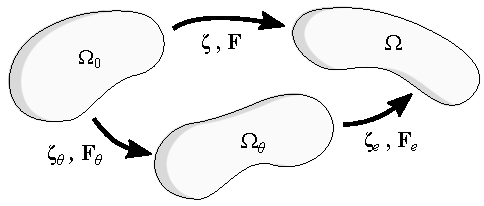
\includegraphics[scale=1.0]{Figuras/termoelastic-kinematics.pdf}
	%\caption*{\textbf{Fonte:} Elaborado pelo autor}
\end{figure}

%Vale ser ressaltado que a decomposição multiplicativa não é única, pois pode ser gerada por qualquer configuração intermediária que resulta de um movimento de corpo rígido em $\domVolt$. Para contornar tal problema, assume-se que a passagem de $\domVolt$ para $\domVol$ envolve apenas deformações puras, isto é, o tensor rotação da decomposição polar de $\Fe$ é a identidade \cite{Khan1995}.

A partir disso, pode-se escrever as parcelas elástica e térmica da deformação de Green-Lagrange, respectivamente, como:
\begin{align}
&\Ee = \dfrac{1}{2}(\Fe^T\Fe-\I) = \dfrac{1}{2}(\Ce-\I) , \label{eq:Ee}\\[0.1cm]
&\Et = \dfrac{1}{2}(\Ft^T\Ft-\I) = \dfrac{1}{2}(\Ct-\I) , \label{eq:Et}
\end{align}
onde, novamente, $\Ee$ é definido na configuração intermediária, enquanto $\Et$ é definido na configuração inicial. Após determinadas manipulações algébricas, pode-se ainda escrever:
\begin{equation}\label{eq:Ee-2}
\Ee = \Ft^{-T}(\E-\Et)\Ft^{-1}.
\end{equation}
Observa-se que, para pequenas deformações térmicas, $\Ft\approx\I$, logo a \cref{eq:Ee-2} se aproxima da decomposição aditiva.

Uma vez que $\Ee$ é definido na configuração intermediária, é natural definir o modelo constitutivo mecânico no mesmo domínio. Dessa forma, denota-se por $\helmholtzmInt$ a parcela mecânica da energia livre de Helmholtz por unidade de volume na configuração intermediária, escrita em função de $\Ee$ conforme os modelos descritos na \autoref{sec:hiper}. Como as demais passagens deste trabalho utilizam a versão Lagrangiana da energia livre, torna-se necessário recupera-la a partir da seguinte expressão:
\begin{equation}\label{eq:psim-int}
\helmholtzm = \Jt\helmholtzmInt,
\end{equation}
onde $\Jt=\det\Ft$ é o Jacobiano da parcela térmica de deformação. O tensor de Piola-Kirchhoff de segunda espécie é dado então por:
\begin{equation}\label{eq:S-termo}
\S = \dfrac{\partial\helmholtzm}{\partial\E} = \Jt\dfrac{\partial\helmholtzmInt}{\partial\Ee}:\dfrac{\partial\Ee}{\partial\E} = \Jt\Ft^{-1}\Se\Ft^{-T},
\end{equation}
onde
\begin{equation}
\Se = \dfrac{\partial\helmholtzmInt}{\partial\Ee}
\end{equation}
é o tensor de Piola-Kirchhoff de segunda espécie definido na configuração intermediária.

A lei de expansão térmica nesse caso pode ser expressa a partir do tensor $\Ft$. Novamente, leva-se em conta que os efeitos térmicos devem ser apenas de dilatação ou contração, logo, apenas as parcelas da diagonal principal de $\Ft$ devem ser não-nulas. Para o caso isotrópico, considerado neste trabalho, escreve-se:
\begin{equation}\label{eq:lei-expansao}
\Ft = \alongTermico\I,
\end{equation}
onde $\alongTermico$ é denominado alongamento térmico, dependente apenas da temperatura. Neste caso, duas leis são consideradas: linear e exponencial. A primeira, dada pela expressão
\begin{equation}\label{eq:expansao-linear-2}
\alongTermico = 1 + \coefExp(\temp-\tempref),
\end{equation}
deve ser utilizada apenas para deformações térmicas pequenas ou moderadas, uma vez que ela permite valores de alongamento inferiores a zero, o que é fisicamente inadmissível. Já a lei exponencial, dada pela expressão
\begin{equation}\label{eq:expansao-exp}
\alongTermico = e^{\coefExp(\temp-\tempref)}
\end{equation}
pode ser utilizada para problemas de grandes deformações sem que hajam inconsistências físicas. Nota-se que, para valores suficientemente pequenos de $\coefExp(\temp-\tempref)$, as duas leis descritas tornam-se coincidentes.

Aplicando a \cref{eq:lei-expansao} nas \cref{eq:Et,eq:Ee-2,eq:psim-int,eq:S-termo}, as relações cinemáticas e constitutivas podem ser reescritas como:
\begin{align}
&\Et = \dfrac{1}{2}(\alongTermico^2-1)\I ,\label{eq:Et-isotropico}\\[0.1cm]
&\Ee = \alongTermico^{-2}\E+\dfrac{1}{2}(\alongTermico^{-2}-1)\I ,\label{eq:Ee-termo-iso}\\[0.1cm]
&\helmholtzm = \alongTermico^3\,\helmholtzmInt, \\[0.1cm]
&\S = \alongTermico\,\Se.
\end{align}
Além disso, pode-se calcular o operador tangente consistente pela expressão:
\begin{equation}
\CC = \dfrac{d\S}{d\E} = \alongTermico\dfrac{d\Se}{d\Ee}:\dfrac{\partial\Ee}{\partial\E}=\dfrac{1}{\alongTermico}\dfrac{d\Se}{d\Ee} = \alongTermico^{-1}\CCe,
\end{equation}
onde
\begin{equation}
\CCe = \dfrac{d \Se}{d \Ee} = \dfrac{d}{d\Ee}\left(\dfrac{\partial \helmholtzm}{\partial\Ee}\right)
\end{equation}
é o operador tangente elástico.

%\subsubsection{Modelo de Saint Venant-Kirchhoff}

Adotando, por exemplo, o modelo de Saint Venant-Kirchhoff para $\helmholtzmInt$, a energia livre de Helmholtz, o tensor de Piola-Kirchhoff de segunda espécie e o operador termo-elástico são dados, respectivamente, por:
\begin{align}
&\helmholtzm = \dfrac{1}{2}\alongTermico^3\,\Ee:\CCSVK:\Ee, \label{eq:helm-svk-mult}\\[0.1cm]
&\S = \alongTermico\,\CCSVK:\Ee, \\[0.1cm]
&\CC = \alongTermico^{-1}\,\CCSVK.
\end{align}
Já para o modelo neo-Hookeano, têm-se:
\begin{align}
&\helmholtzm = \dfrac{\alongTermico^3\lame}{2}\ln(\Je)^2 + \dfrac{\alongTermico^3\G}{2}\left(\tr\Ce - 3 - 2\ln\Je\right), \\[0.1cm]
&\S = \alongTermico\lame\ln(\Je)\Ce^{-1} + \alongTermico\G(\I-\Ce^{-1}), \\[0.1cm]
&\CC = \alongTermico^{-1}\lame\Ce^{-1}\otimes\Ce^{-1}+2\alongTermico^{-1}\lame\ln(\Je)\dfrac{\partial\Ce^{-1}}{\partial\Ce^{\;\;}} - 2\alongTermico^{-1}\G\dfrac{\partial\Ce^{-1}}{\partial\Ce^{\;\;}}.
\end{align}
%Derivando a \cref{eq:helm-svk-mult} com relação à temperatura, temos:
%\begin{equation}
%\dfrac{\partial\helmholtzm}{\partial\temp} = \left(\dfrac{\partial\helmholtzm}{\partial\alongTermico} + \dfrac{\partial\helmholtzm}{\partial\Ee}:\dfrac{\partial\Ee}{\partial\alongTermico}\right)\dfrac{\partial\alongTermico}{\partial\temp} = -\dfrac{1}{4}(\CCSVK:\Ee):\left(\C+3\alongTermico^2\,\I\right)\dfrac{\partial\alongTermico}{\partial\temp},
%\end{equation}
%de onde, compondo com a \cref{eq:entropiat}, pode-se obter a entropia:
%\begin{equation}
%\massi\entropy = \dfrac{1}{4}(\CCSVK:\Ee):\left(\C+3\alongTermico^2\,\I\right)\dfrac{\partial\alongTermico}{\partial\temp}-(\specificHeatIni-\specificHeatConst\tempref)\ln\left(\dfrac{\tempref}{\temp}\right)+\specificHeatConst(\temp-\tempref).
%\end{equation}
%A partir da entropia, podemos obter as seguintes expressões para o operador termo-elástico e o calor específico:
%\begin{align}
%&\operadorTermoElastico = \massi\dfrac{\partial\entropy}{\partial\E} = \CCSVK:\left[\alongTermico^{-2}\E+\dfrac{1}{2}(\alongTermico^{-2}+1)\I\right]\dfrac{\partial\alongTermico}{\partial\temp} \\[0.1cm]
%&\specificHeat = \massi\temp\dfrac{\partial\entropy}{\partial\temp} = \specificHeatIni+\specificHeatConst(\temp - \tempref) - \coefExp\temp\,\I:(\CC-\CCtNeg):\I.
%\end{align}

A derivada de $\helmholtzm$ com relação à temperatura pode ser escrita como:
\begin{equation}
\dfrac{\partial\helmholtzm}{\partial\temp} = \dfrac{\partial(\alongTermico^3\helmholtzmInt)}{\partial\alongTermico}\dfrac{\partial\alongTermico}{\partial\temp} = \left(3\alongTermico^2\helmholtzmInt-\Se:\C\right)\dfrac{\partial\alongTermico}{\partial\temp},
\end{equation}
de forma que, aplicando a \cref{eq:const2}, obtém-se a seguinte expressão para a entropia:
\begin{equation}
\entropy = \left(\Se:\C-3\alongTermico^2\helmholtzmInt\right)\dfrac{\partial\alongTermico}{\partial\temp}-(\specificHeatIni-\specificHeatConst\tempref)\ln\left(\dfrac{\tempref}{\temp}\right)+\specificHeatConst(\temp-\tempref).
\end{equation}
A partir dessa equação, podem ser obtidas as seguintes expressões para o operador termo-elástico e para o calor específico volumétrico:
\begin{align}
&\operadorTermoElastico = \dfrac{\partial\entropy}{\partial\E} = \left(\alongTermico^{-2}\CCe:\C - \Se\right)\dfrac{\partial\alongTermico}{\partial\temp}, \\[0.1cm]
&\volumetricHeatCapacity = \temp\dfrac{\partial\entropy}{\partial\temp} = \specificHeatIni+\specificHeatConst(\temp - \tempref) + \temp\left(\Se:\C-3\alongTermico^2\helmholtzmInt\right)\dfrac{\partial^2\alongTermico}{\partial\temp^2} \\
&\phantom{\specificHeat = \massi\temp\dfrac{\partial\entropy}{\partial\temp} =}+ \temp\left(-\alongTermico^{-3}\C:\CCe:\C-6\alongTermico\helmholtzmInt+3\alongTermico^{-1}\Se:\C\right)\left(\dfrac{\partial\alongTermico}{\partial\temp}\right)^2.
\end{align}

O termo $\partial^2\alongTermico/\partial\temp^2$ será anulado para a lei de expansão térmica linear, e será da ordem de $\coefExp^2$ para a lei exponencial. Já o termo $(\partial\alongTermico/\partial\temp)^2$ será da ordem de $\coefExp^2$ independente da lei adotada. Portanto, admitindo novamente a hipótese $\coefExp \ll \volumetricHeatCapacity$, esses termos podem ser desprezados, e o calor específico pode ainda ser escrito conforme a expressão \eqref{eq:psim-int}.

%\subsubsection{Modelo neo-Hookeano}
%
%Já para o modelo neo-Hookeano:
%\begin{align}
%&\helmholtzm = \dfrac{\alongTermico^3\lame}{2}\ln(\Je)^2 + \dfrac{\alongTermico^3\G}{2}\left(\tr\Ce - 3 - 2\ln\Je\right), \\[0.1cm]
%&\S = \alongTermico\lame\ln(\Je)\Ce^{-1} + \alongTermico\G(\I-\Ce^{-1}), \\[0.1cm]
%&\CC = \alongTermico^{-1}\lame\Ce^{-1}\otimes\Ce^{-1}+2\alongTermico^{-1}\lame\ln(\Je)\dfrac{\partial\Ce^{-1}}{\partial\Ce^{\;\;}} - 2\alongTermico^{-1}\G\dfrac{\partial\Ce^{-1}}{\partial\Ce^{\;\;}}.
%\end{align}

\subsection{Equivalência entre leis de expansão térmica}\label{sec:equivalencia-leis-expansao}

Neste trabalho, serão aplicadas as leis de expansão térmica linear e exponencial, definidas conforme as \cref{eq:expansao-linear-2,eq:expansao-exp} para o modelo baseado na decomposição multiplicativa. Para aplicar essas mesmas leis na decomposição aditiva, e possibilitar uma comparação justa entre as duas abordagens, deve-se levar em conta que elas são escritas em termos de $\Et$ ao invés de $\alongTermico$, sendo necessário utilizar a \cref{eq:Et-isotropico} para relacioná-las. Portanto, aplicando nessa as \cref{eq:expansao-linear-2,eq:expansao-exp}, pode-se escrever as leis linear e exponencial, respectivamente, como:
\begin{align}
&\Et = \left[\coefExp(\temp-\tempref) + \dfrac{1}{2}\coefExp^2(\temp-\tempref)^2\right]\I, \text{\;e} \label{eq:expansao-linear-3}\\[0.1cm]
&\Et = \dfrac{1}{2}(e^{2\coefExp(\temp-\tempref)}-1)\I. \label{eq:expansao-exp-2}
\end{align}

Observa-se que a lei linear para o alongamento retorna quadrática para o tensor de deformações de Green-Lagrange, ao contrário da lei definida na \cref{eq:expansao-linear}. Naturalmente, considerando a hipótese $\coefExp\ll 1$, o segundo termo da \cref{eq:expansao-linear-3} é desprezível comparado ao primeiro, fazendo com que as duas leis sejam aproximadamente coincidentes. No entanto, a fim de abordar o caso geral, neste trabalho apenas a \cref{eq:expansao-linear-3} será considerada para a lei linear.

%\subsection{Estados planos de tensão e deformação}
%
%Para aplicar o modelo constitutivo termo-elástico em problemas bidimensionais, as aproximações do EPD e EPT, discutidas na \autoref{subsec:estado-plano}, podem ser utilizadas. No entanto, algumas considerações devem ser feitas

\section{Equação termo-elástica da condução de calor}\label{sec:conducao-calor}

Para se obter a forma variacional global da equação da condução de calor para o caso termo-elástico, pode-se aplicar procedimentos algébricos análogos aos realizados na \autoref{sec:conducao-calor-0}, partindo da sua forma local apresentada na \cref{eq:equacao-conducao-local}. Aplicando-se também a lei de Fourier, de forma análoga à \autoref{subsec:fourier-0}, temos:
\begin{equation}\label{eq:equacao-conducao-global-fourier}
\begin{aligned}
&\int_{\domVoli}\left(\condutMati\cdot\gradientei\,\temp\right)\cdot\left(\gradientei\,\delta\temp\right) d\voli + \int_{\domVoli}\volumetricHeatCapacity\dottemp\delta\temp d\voli + \int_{\domConi}\qpresci\,\delta\temp d\coni \\&- \int_{\domVoli}\calorInt\delta\temp d\voli + \int_{\domVoli}\temp\operadorTermoElastico:\dotE\,\delta\temp d\voli = 0.
\end{aligned}
\end{equation}

Nota-se que a única diferença entre a \cref{eq:equacao-conducao-global-fourier} e a \cref{eq:equacao-conducao-global-fourier-term} é a adição do termo associado ao operador termo-elástico $\operadorTermoElastico$. No entanto, como será mencionado a seguir, esse termo geralmente possui ordem de grandeza muito inferior aos demais, sendo portanto desconsiderado nos exemplos deste capítulo.

\section{Solução numérica da termo-elasticidade}\label{sec:solucao-numerica-termo-elasticidade}

A solução numérica do problema térmico é dada novamente pelo Método dos Elementos Finitos, conforme descrito na \autoref{sec:mef-termo}. Apesar de terem sido apresentadas equações gerais em muitas passagens deste capítulo, a aplicação numérica do problema termo-mecânico limita-se a algumas aproximações e considerações importantes:
\begin{enumerate}%[topsep=1pt,itemsep=0.5ex,partopsep=1pt,parsep=1pt]
	\item Modelos adotados são isotrópicos, isto é, $\boldsymbol{\coefExp} = \coefExp\I$, $\condutMat = \condut\I$ e $\condutMati = \condut\J\C^{-1}$.
	\item Coeficiente de expansão térmica é pequeno, isto é, $\coefExp\ll 1$. Como consequência:
	\begin{itemize}%[nolistsep]
		\item Os termos do calor específico que dependem das deformações são desprezados, por apresentarem ordem de grandeza muito inferior à constante $\specificHeatIni$;
		\item O termo do operador termo-elástico, $\operadorTermoElastico$, na equação da condução de calor é desprezado, por apresentar ordem de grandeza muito inferior aos demais termos.
	\end{itemize}
	\item O calor específico é tomado como constante, isto é, $\specificHeatConst = 0$ e $\volumetricHeatCapacity=\specificHeatIni$.
\end{enumerate}

\subsection{Acoplamento termo-mecânico}\label{subsec:acoplamento}

Apesar de apresentarem equações governantes diferentes, os problemas térmico e mecânico são mutuamente dependentes. A variação de temperatura causa dilatação ou contração no material, interferindo no problema mecânico por meio do modelo constitutivo. Já as deformações do corpo interferem no problema térmico de duas formas: a primeira é pelo termo de acoplamento termo-elástico ($\temp\operadorTermoElastico:\dotE$), que, embora desprezado neste trabalho, pode influenciar de forma mais significativa em casos específicos. Já a segunda se deve ao fato de que, quando o corpo é deformado, o gradiente da temperatura é modificado, alterando o fluxo de calor pela lei de Fourier. Esse último fato normalmente é desconsiderado na termo-elasticidade linear, pois a variação é desprezível em problemas de pequenas deformações. No entanto, como este trabalho trata de problemas em grandes deformações, cuidados maiores são tomados nesse sentido.

O acoplamento termo-mecânico podem ser resolvido numericamente de duas formas: monolítica e particionada. No acoplamento monolítico, as incógnitas do problema térmico e do problema mecânico (temperaturas e posições) são resolvidas conjuntamente em um sistema único. Nesse caso, apenas um processo iterativo é necessário, porém, para garantir a convergência, a linearização de ambas as equações governantes deve ser feita com relação à ambos os parâmetros nodais (temperaturas e posições), o que pode resultar em equações relativamente mais complexas e sistemas não-simétricos. 

Já no acoplamento particionado, os problemas térmico e mecânico são resolvidos isoladamente, com trocas de informação feitas de forma explícita ou implícita durante o processo de solução dos sistemas. Na forma explícita, também chamada de acoplamento fraco, a troca de informações é feita apenas uma vez em cada passo de tempo, isto é, resolve-se o problema térmico com as posições do passo anterior, em seguida resolve-se o problema mecânico com as temperaturas previamente calculadas, e parte-se para o próximo passo de tempo. Já na forma implícita, também chamada de acoplamento forte, ou método bloco-iterativo, esse procedimento é realizado a cada iteração do procedimento de solução dos sistemas não lineares, dentro do mesmo passo de tempo, até que a variação das temperaturas e posições sejam menores que uma tolerância pré-estabelecida.

Neste trabalho, aplica-se o acoplamento particionado forte por ter uma implementação mais simples quando comparado ao monolítico e produzir resultados mais confiáveis quando comparado ao particionado fraco. Na \autoref{fig:acoplamento} é apresentado um fluxograma resumido do processo bloco-iterativo adotado.

\begin{figure}[!htb]
	\centering
	\caption{Esquema de acoplamento bloco-iterativo para o problema termo-elástico}
	\label{fig:acoplamento}
	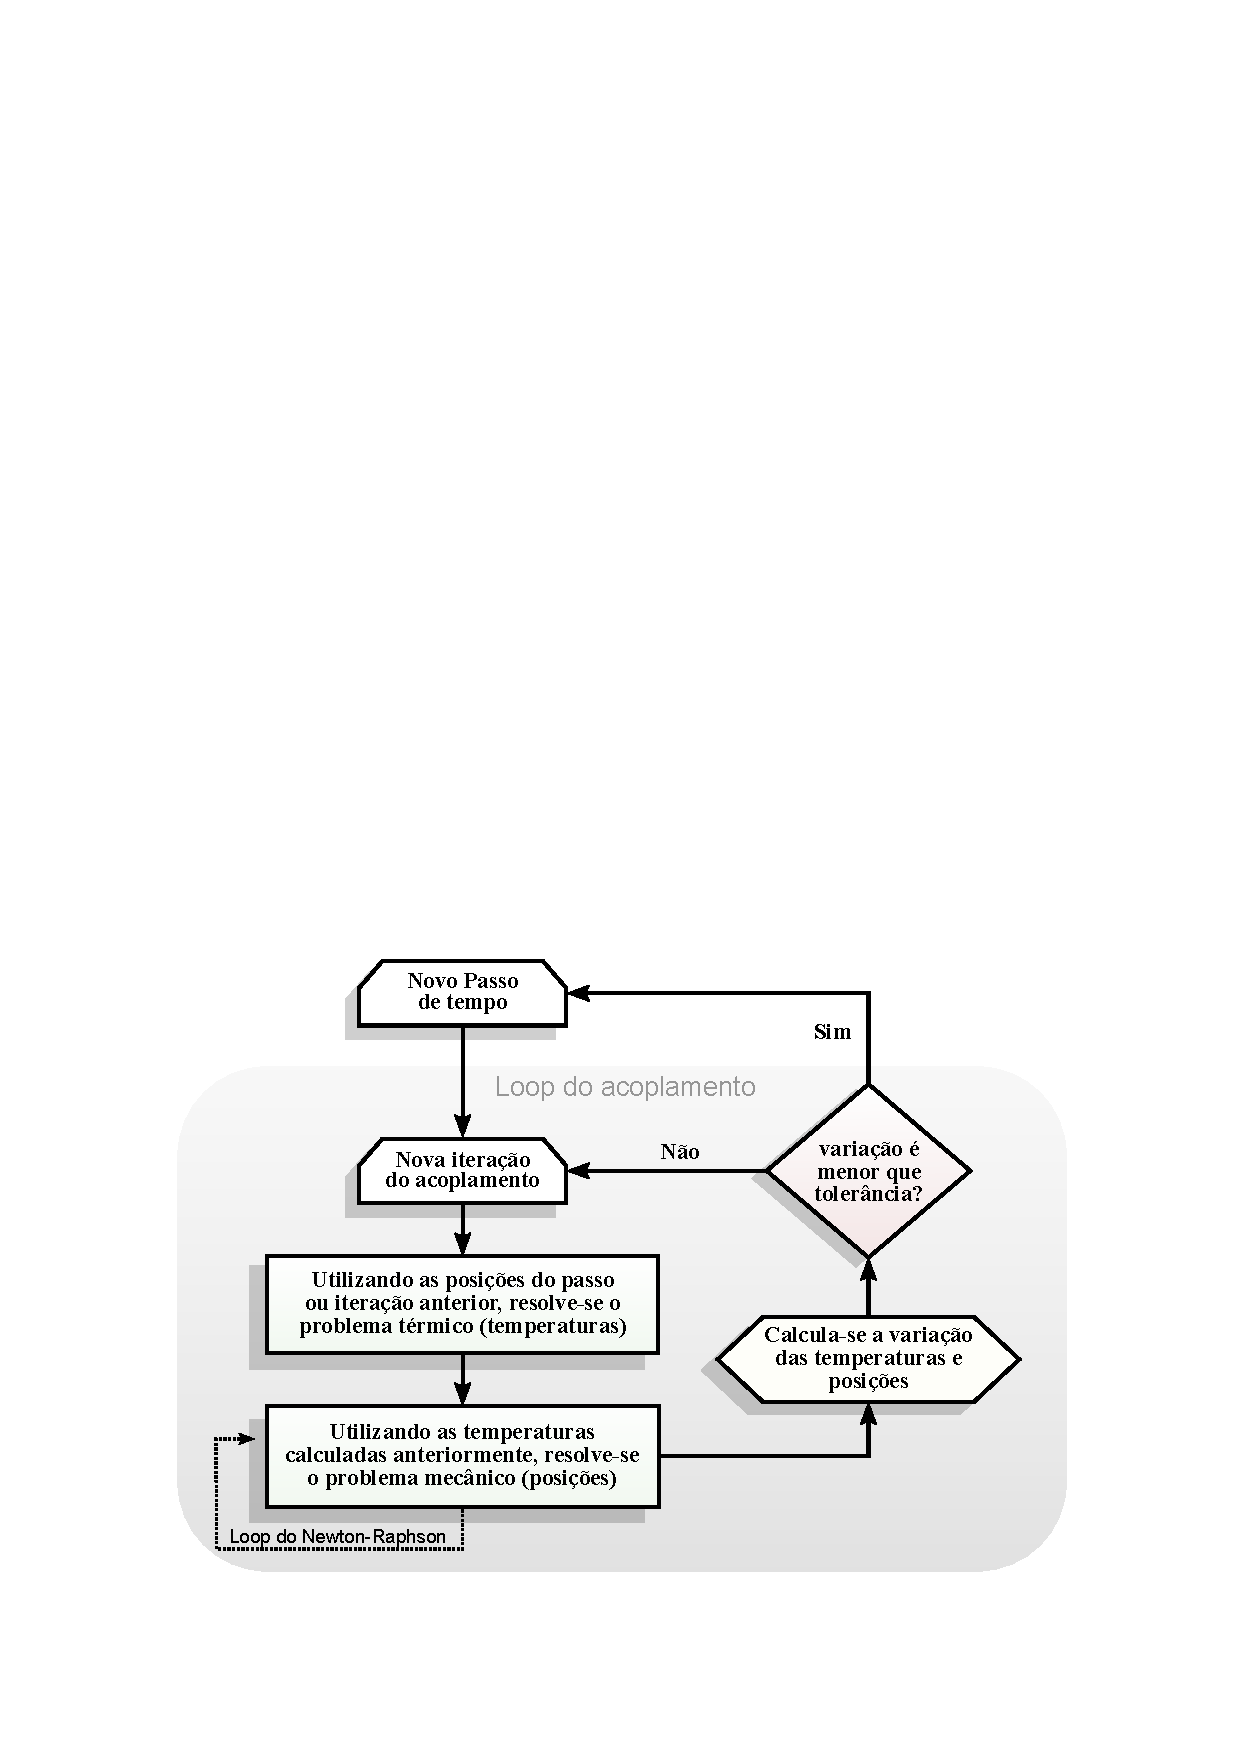
\includegraphics[scale=0.85]{Figuras/acoplamento.pdf}
	%\caption*{\textbf{Fonte:} Elaborado pelo autor}
\end{figure}

\section{Exemplos numéricos}\label{sec:exemplos-termo}

Nesta seção, são apresentados exemplos numéricos de termo-elasticidade com o intuito de verificar o código desenvolvido e comparar os diferentes modelos propostos. Embora a formulação de elementos finitos implementada contemple o caso tridimensional, por simplicidade e menor custo computacional, apenas problemas bidimensionais foram considerados nesta seção. Dessa forma, assume-se que as temperaturas são constantes ao longo do terceiro eixo, e toma-se espessura unitária em todos os exemplos. 

Com relação ao modelo constitutivo mecânico, aplicam-se os estados planos de tensão e de deformação, conforme discutidos na \autoref{subsec:estado-plano}. O EPD neste caso é considerado a partir das deformações totais ao invés das deformações elásticas, isto é, toma-se $\Eind_{33}=0$. Isso implica, para o caso da decomposição aditiva, que $\Eeind_{33}=-\Etind_{33}$ e, para o caso da decomposição multiplicativa, que $\Eeind_{33}=-\alongTermico^{-2}\Etind_{33}$. Com relação ao EPT, nenhuma consideração precisa ser feita além do que foi discutido na \autoref{subsec:estado-plano}.

\subsection{Cubo parcialmente comprimido sob efeitos térmicos}\label{subsec:thermoCube}

Este exemplo é proposto com o intuito de verificar a influência dos carregamentos mecânicos sobre os campos térmicos em problemas com grandes deformações. Considera-se um cubo de dimensões unitárias composto por material sólido, submetido a um fluxo de calor uniforme na face superior, fluxo de calor nulo nas faces da esquerda e da direita e temperatura prescrita na face inferior, além de ser parcialmente carregado por uma força distribuída vertical uniforme na face superior, estando com o deslocamento na direção normal restrito tanto na face inferior quanto na face da direita, como mostra a \autoref{fig:ThermoCube} \textcolor{red}{verifique se o que eu escrevi está correto. Tente descrever melhor o problema no texto.}. As propriedades físicas assim e a discretização espacial também são apresentadas na  \autoref{fig:ThermoCube}, sendo que os carregamentos térmicos são tomados constantes ao longo do tempo, enquanto o carregamento mecânico é incrementado à medida que avança o número de passos. Para que não haja influência do problema térmico no mecânico, desconsideram-se os efeitos da expansão térmica. Além disso, assume-se que o processo seja suficientemente lento para que o problema mecânico possa ser tratado por uma análise estática, e o problema térmico por um regime permanente (considerado no código tomando $\specificHeat=0$).

\begin{figure}[!htb]
	\centering
	\caption{Dados do exemplo de cubo parcialmente comprimido sob efeitos térmicos}
	\label{fig:ThermoCube}
	{\small
		\noindent\shadowbox{
			\parbox{15.3cm}{
				\setlength{\columnseprule}{1pt}
				\vspace{-0.4cm}
				{\centering\begin{center}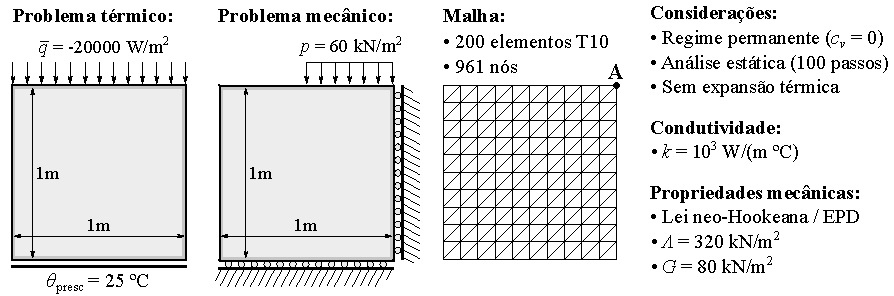
\includegraphics[scale=1.0]{Figuras/ThermoCube/ThermoCube.pdf}\end{center}\par}
				\vspace{-0.4cm}
			}
		}
	}	
	%\caption*{\textbf{Fonte:} Elaborado pelo autor}
\end{figure}

Caso sejam desconsiderados os efeitos mecânicos, pode-se facilmente resolver o problema térmico de forma analítica, aplicando de forma direta a lei de Fourier para obter a temperatura no topo do corpo ($\temp_\text{topo}$):
\begin{equation}\label{eq:solucao-problem-term-1}
\qpresc = -\condut\dfrac{(\temp_\text{topo}-\temp_\text{presc})}{h} \Rightarrow -20000 = -1000\cdot(\temp_\text{topo}-25) \Rightarrow \temp_\text{topo} = 45^{\circ}\text{C}.
\end{equation}
Essa solução reflete de forma aproximada as temperaturas obtidas nos primeiros passos do problema, como pode ser visto nos resultados do primeiro passo, apresentados na \autoref{fig:ThermoCube-resp}. No entanto, ainda na \autoref{fig:ThermoCube-resp}, pode-se observar a variação no campo de temperatura do último passo, decorrente do surgimento de deformações modificando o gradiente de temperatura.

\begin{figure}[!htb]
	\centering
	\caption{Configuração deformada e campo de temperatura (em $^{\circ}$C) para o primeiro e último passo do carregamento mecânico}
	\label{fig:ThermoCube-resp}
	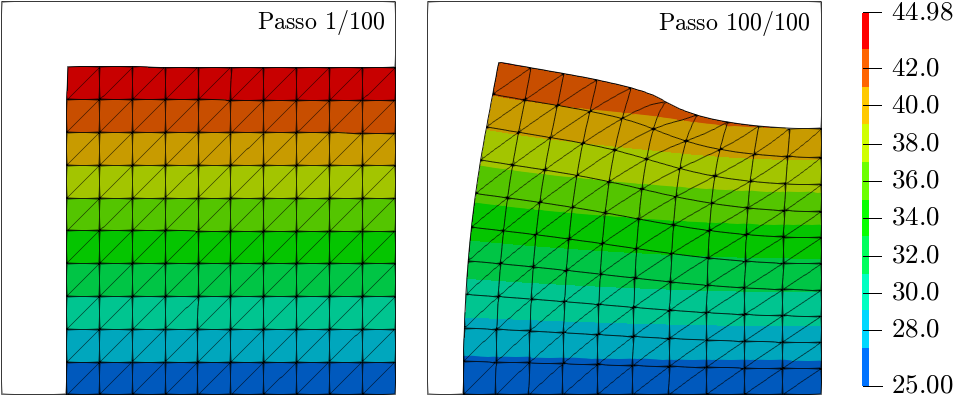
\includegraphics[scale=0.45]{Figuras/ThermoCube/ThermoCube.png}
	%\caption*{\textbf{Fonte:} Elaborado pelo autor}
\end{figure}

Na \autoref{fig:termoCube-graphs} são apresentados os gráficos de deslocamento vertical e temperatura no canto superior direito (ponto A) do corpo, onde são comparados com resultados obtidos por meio do \emph{software} ANSYS, mostrando concordância satisfatória. Observa-se que a temperatura parte da solução puramente térmica esperada ($45^{\circ}$C) e varia conforme o nível de deformação aumenta, até um valor limite de aproximadamente $41^{\circ}$C. Essa variação é possível pois a constante de condutividade térmica foi tomada na sua forma Euleriana, ao invés da Lagrangiana, conforme comentado na \autoref{subsec:fourier-0}.

\begin{figure*}[!htb]
	\centering
	\caption{Deslocamento e temperatura vs. tempo no ponto A}
	\label{fig:termoCube-graphs}
	\makebox[\textwidth]{
		\captionsetup[subfigure]{aboveskip=-0.6pt,belowskip=-0.7pt}
		\begin{subfigure}{8.1cm}
			\centering
			\subcaption{}
			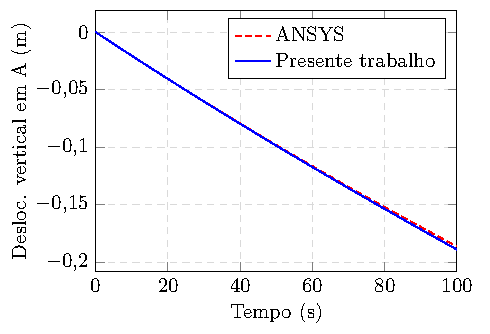
\includegraphics[scale=1.0]{Figuras/ThermoCube/v.pdf}			
		\end{subfigure}%7
		\begin{subfigure}{8.1cm}
			\centering
			\subcaption{}
			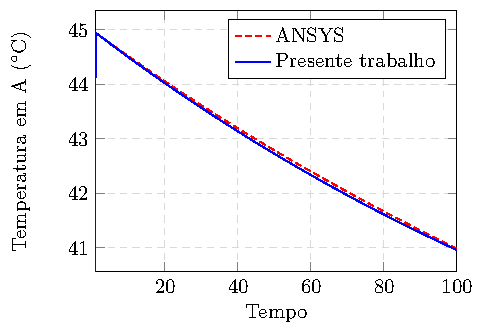
\includegraphics[scale=1.0]{Figuras/ThermoCube/temp.pdf}			
		\end{subfigure}
	}	
	%\caption*{\textbf{Fonte:} Elaborado pelo autor}	
\end{figure*}


\subsection{Viga biapoiada sujeita a variação de temperatura}\label{subsec:thermoBeam}

Neste exemplo, observa-se o efeito da expansão térmica e dos diferentes modelos constitutivos termo-elásticos no comportamento do corpo. Considera-se uma viga biapoiada sujeita à variação de temperatura negativa na borda superior e positiva na borda inferior, de forma que o efeito esperado seja de flexão, deslocando o centro do vão para baixo. Assume-se novamente análise estática e regime permanente, com as variações de temperatura sendo incrementadas a cada passo da análise. Ambas as decomposições, aditiva e multiplicativa, foram consideradas neste problema, e em cada uma foram adotadas as leis de expansão térmica linear e exponencial, totalizando quatro casos a serem analisados. Todos os dados do problema, incluindo geometria, condições de contorno, propriedades físicas e discretização, estão dispostos na \autoref{fig:ThermoBeam1}.

\begin{figure}[!htb]
	\centering
	\caption{Dados do exemplo de viga biapoiada sujeita a variação de temperatura}
	\label{fig:ThermoBeam1}
	{\small
		\noindent\shadowbox{
			\parbox{15.3cm}{
				\setlength{\columnseprule}{1pt}
				\vspace{-0.4cm}
				{\centering\begin{center}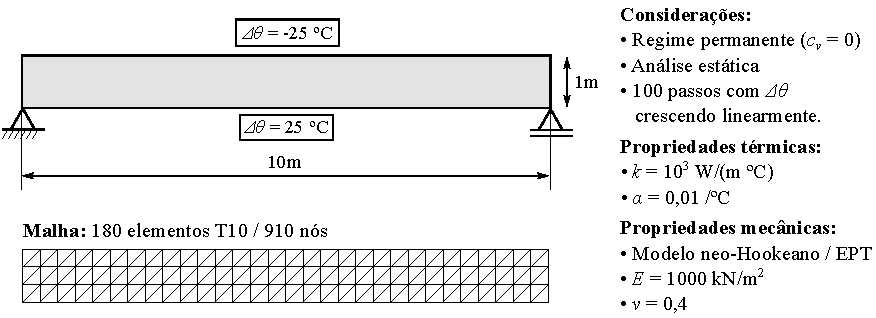
\includegraphics[scale=1.03]{Figuras/ThermoBeam/ThermoBeam1.pdf}\end{center}\par}
				\vspace{-0.4cm}
			}
		}
	}	
	%\caption*{\textbf{Fonte:} Elaborado pelo autor}
\end{figure}

Por se tratar de uma viga isostática, sujeita apenas a carregamentos térmicos, sabe-se que as reações de apoio mecânicas devem ser nulas, assim como as componentes de tensão.\textcolor{green}{ No entanto, isso não impede que se manifestem tensões residuais no domínio da viga, decorrentes de incompatibilidades entre as deformações puramente térmicas e os deslocamentos, que são compensadas com o surgimento de deformações elásticas.} \textcolor{red}{O que você quer dizer com residual nesse contexto? Deixe isso claro aqui.}
Na \autoref{fig:ThermoBeamStress}, apresenta-se a componente $\cauchyind_{11}$ das tensões de Cauchy para o último passo de tempo em cada um dos casos analisados. Observa-se que as tensões residuais são evidentes apenas nos casos onde foi adotada a lei de expansão térmica linear. Para a lei exponencial, as tensões obtidas (e, portanto, as deformações elásticas) são desprezíveis, demonstrando que essa permite uma mais adequada compatibilização das deformações puramente térmicas.

\begin{figure}[!htb]
	\centering
	\caption{Componente $\cauchyind_{11}$ da tensão de Cauchy no último passo do exemplo de viga biapoiada sujeita a variação de temperatura, utilizando (a) decomposição aditiva com lei de expansão térmica linear, (b) decomp. aditiva com lei exponencial, (c) decomp. multiplicativa com lei linear e (d) decomp. multiplicativa com lei exponencial}
	\label{fig:ThermoBeamStress}
	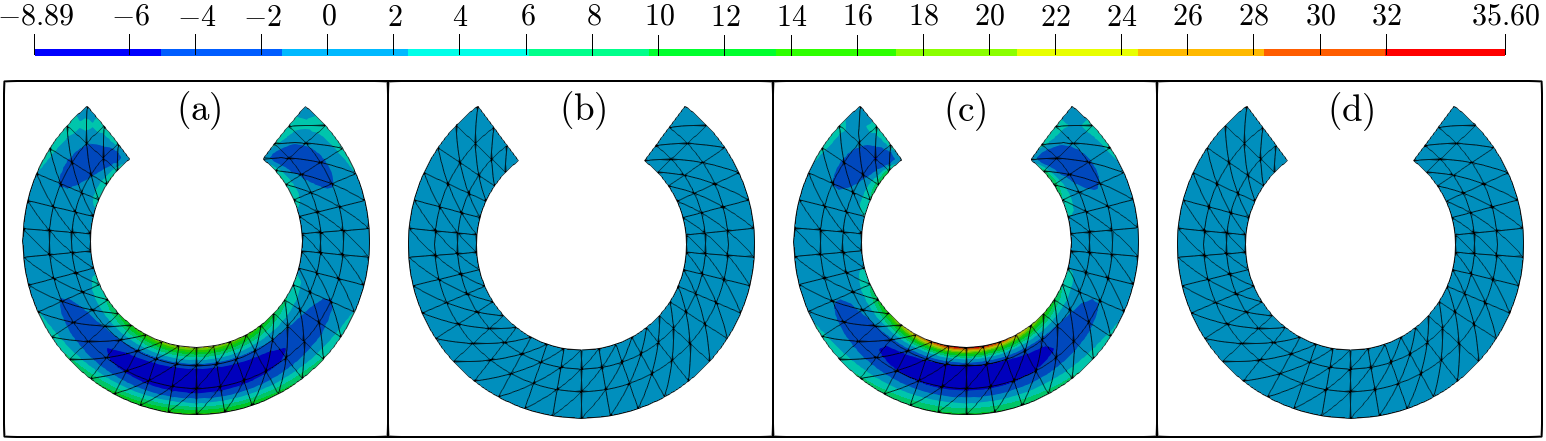
\includegraphics[scale=0.39]{Figuras/ThermoBeam/ThermoBeamStress.png}
	%\caption*{\textbf{Fonte:} Elaborado pelo autor}
\end{figure}

\textcolor{red}{precisa identificar o eixo 1 relativo a $\sigma_{11}$! É tensão de Cauchy segundo o eixo horizontal (reto), ou segundo o eixo da viga deformado? Porque com a Lei linear surgem tensões? é só a componente 11 que fica diferente de zero? O mesmo vale para o próximo exemplo.}
Pelo fato de as deformações elásticas neste problema serem residuais, isto é, as deformações totais consistirem praticamente de suas parcelas térmicas, espera-se que não haja diferenças significativas entre as decomposições aditiva e multiplicativa. Essa expectativa é confirmada pelos resultados da \autoref{fig:v}, onde são apresentados os gráficos de deslocamento e deformação na borda inferior do meio do vão. Embora diferenças entre as leis de expansão linear e exponencial sejam notáveis, especialmente na \autoref{fig:v}(b), observa-se que em cada uma delas a escolha da decomposição de fato não manifesta um papel significativo. Mesmo no gráfico ampliado da \autoref{fig:v}(a), só é possível observar diferenças mínimas para o caso da lei linear, onde as deformações residuais são maiores.

\begin{figure}[!htb]
	\centering
	\caption{Gráficos de (a) deslocamento vertical e (b) componente $\Eind_{11}$ da deformação, calculados na borda inferior do meio do vão para o exemplo de viga biapoiada sujeita a variação de temperatura}
	\label{fig:v}
	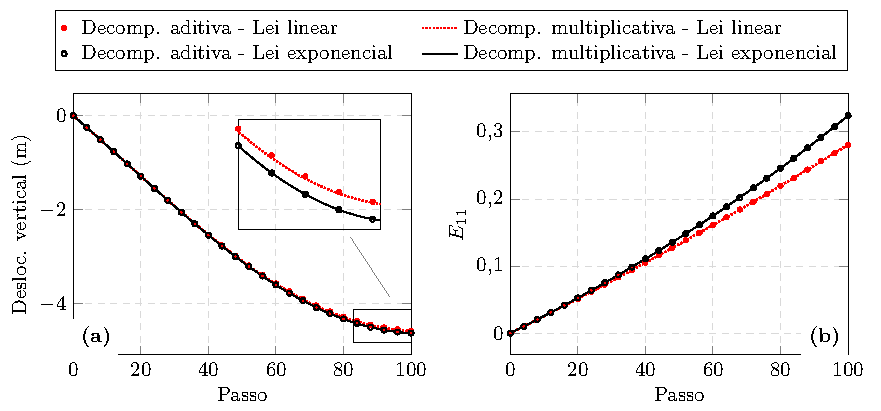
\includegraphics[scale=1.1]{Figuras/ThermoBeam/v.pdf}
	%\caption*{\textbf{Fonte:} Elaborado pelo autor}
\end{figure}

\subsection{Viga biapoiada sujeita a variação de temperatura e carregamento mecânico}\label{subsec:thermoBeam2}

Com o intuito de aumentar a influência das deformações elásticas, o exemplo anterior é reformulado nesta subseção, sendo adicionado um carregamento mecânico distribuído ao longo do vão, e reduzidas as variações de temperatura. Os dados são apresentados na \autoref{fig:ThermoBeam2}.

\begin{figure}[!htb]
	\centering
	\caption{Dados do exemplo de viga biapoiada sujeita a variação de temperatura e carregamento mecânico}
	\label{fig:ThermoBeam2}
	{\small
		\noindent\shadowbox{
			\parbox{15.3cm}{
				\setlength{\columnseprule}{1pt}
				\vspace{-0.2cm}
				{\centering\begin{center}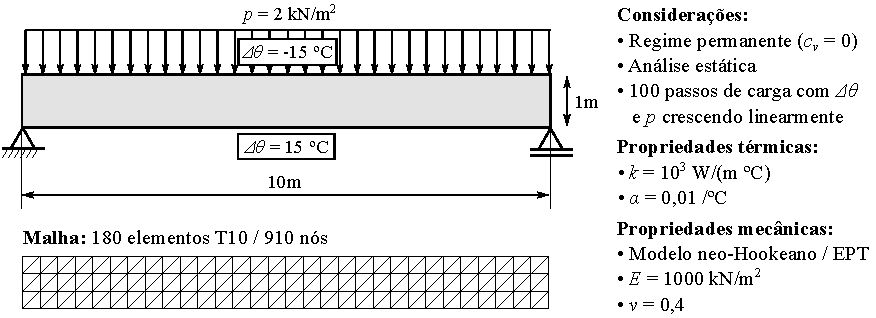
\includegraphics[scale=1.03]{Figuras/ThermoBeam/ThermoBeam2.pdf}\end{center}\par}
				\vspace{-0.2cm}
			}
		}
	}	
	%\caption*{\textbf{Fonte:} Elaborado pelo autor}
\end{figure}

Como consequência das deformações mecânicas decorrentes do carregamento aplicado, o campo das componentes horizontais de tensão deixa de ser residual e apresenta a disposição mostrada na \autoref{fig:ThermoBeamStressLoad}. Além disso, a própria configuração deformada diferencia-se do caso anterior, apresentando um formato ligeiramente menos circular pelo fato de as deformações serem maiores no meio do vão.

\begin{figure}[!htb]
	\centering
	\caption{Componente $\cauchyind_{11}$ da tensão de Cauchy no último passo do exemplo de viga biapoiada sujeita a variação de temperatura e carregamento mecânico, utilizando (a) decomposição aditiva com lei de expansão térmica linear, (b) decomp. aditiva com lei exponencial, (c) decomp. multiplicativa com lei linear e (d) decomp. multiplicativa com lei exponencial}
	\label{fig:ThermoBeamStressLoad}
	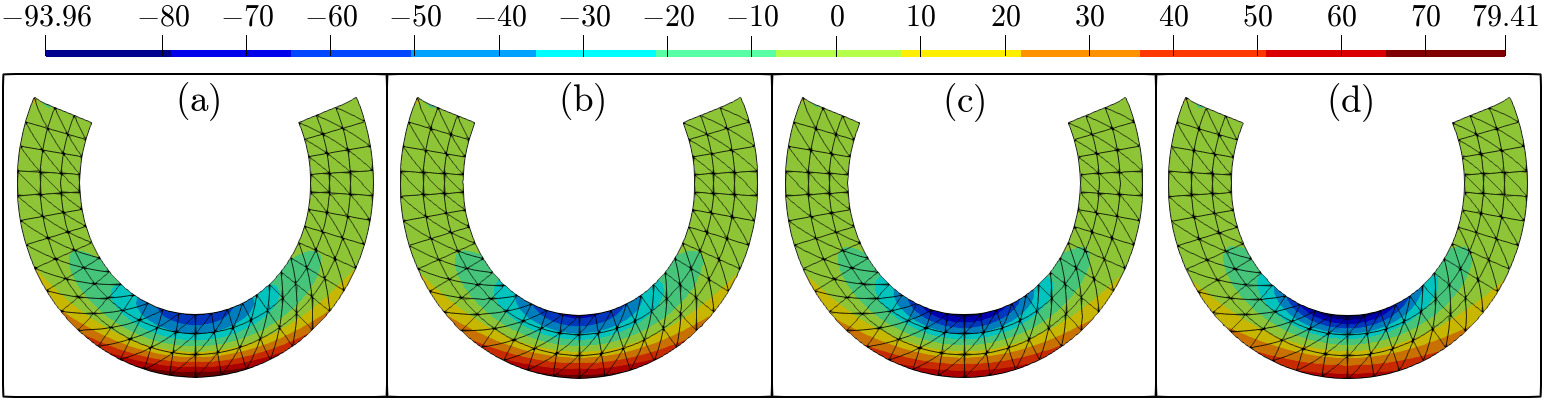
\includegraphics[scale=0.39]{Figuras/ThermoBeam/ThermoBeamStress-Load.png}
	%\caption*{\textbf{Fonte:} Elaborado pelo autor}
\end{figure}

Outra consequência do acréscimo nas deformações elásticas é a maior diferença entre as decomposições aditiva e multiplicativa, conforme atestado nos gráficos da \autoref{fig:v-Load}. De fato, ao contrário do caso sem carregamento mecânico, é notável a variação entre os valores obtidos para os dois tipos de decomposição, principalmente na \autoref{fig:v-Load}(b). No entanto, pelo fato de as deformações térmicas neste caso serem menores, as diferenças entre as leis de expansão térmica adotadas não são tão expressivas quanto as observadas no exemplo anterior.

\begin{figure}[!htb]
	\centering
	\caption{Gráficos de (a) deslocamento vertical e (b) componente $\Eind_{11}$ da deformação, calculados na borda inferior do meio do vão para o exemplo de viga biapoiada sujeita a variação de temperatura e carregamento mecânico}
	\label{fig:v-Load}
	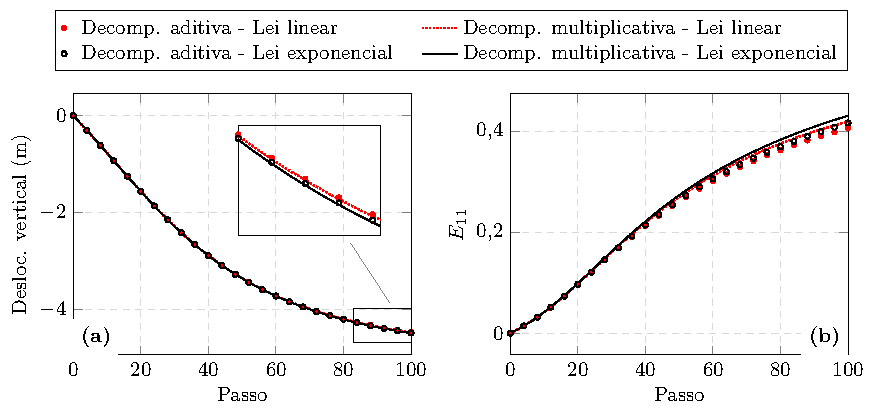
\includegraphics[scale=1.1]{Figuras/ThermoBeam/v-Load.pdf}
	%\caption*{\textbf{Fonte:} Elaborado pelo autor}
\end{figure}

\subsection{Cubo sob deformações térmicas excessivas}\label{subsec:thermoCube2}

Este exemplo é proposto para verificar a influência do modelo adotado em problemas de grandes deformações. Considera-se um cubo de dimensões unitárias previamente aquecido a uma temperatura de $600\text{ }^{\circ}$C, submetido a uma temperatura ambiente de $25\text{ }^{\circ}$C e condição de convecção em todas as faces. O coeficiente de expansão é escolhido de forma que essa variação de temperatura provoque um alto valor de contração térmica. No entanto, o corpo é restrito mecanicamente tanto em sua largura quanto em sua profundidade (EPD), de forma que a deformação seja livre apenas na direção vertical. O problema térmico é considerado transiente, com tempo máximo de análise $100$ s, e $\Delta t = 0,25$ s. Já o problema mecânico é resolvido desprezando-se as parcelas dinâmicas (análise estática). Os demais dados do problema são dispostos na \autoref{fig:ThermoBeam3}.

\begin{figure}[!htb]
	\centering
	\caption{Cubo sob deformações térmicas excessivas - Descrição do problema e da discretização}
	\label{fig:ThermoBeam3}
	{\small
		\noindent\shadowbox{
			\parbox{15.3cm}{
				\setlength{\columnseprule}{1pt}
				\vspace{-0.3cm}
				{\centering\begin{center}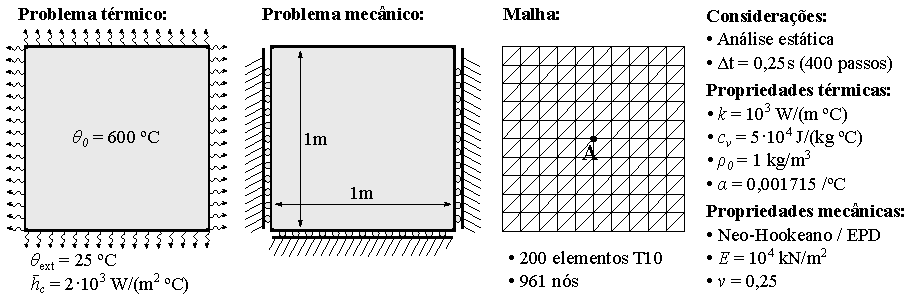
\includegraphics[scale=1.0]{Figuras/ThermoCube3/ThermoCube3.pdf}\end{center}\par}
				\vspace{-0.3cm}
			}
		}
	}	
	%\caption*{\textbf{Fonte:} Elaborado pelo autor}
\end{figure}

Novamente, são aplicados os modelos baseados nas decomposições aditiva e multiplicativa e as leis de expansão térmica linear e exponencial. Dessas quatro combinações, o único modelo capaz de prosseguir até o final da análise foi o de decomposição multiplicativa com lei exponencial. Os demais apresentaram problema de inversão do material (Jacobiano negativo), devido às já mencionadas limitações quando submetidos a altos níveis de deformações compressivas. Para o caso de decomposição multiplicativa com lei de expansão térmica linear, houve erro de convergência \textcolor{red}{no processo iterativo de solução do sistema não linear?} no passo $151$ ($t=37,75$s); para o caso de decomposição aditiva com lei exponencial, no passo 34 ($t=8,5$s); para o caso de decomposição aditiva com lei linear, no passo 11 ($t=2,75$s).

Na \autoref{fig:ThermoCube3Results} são apresentados os gráficos de temperatura, alongamento térmico, e componentes horizontal e vertical da deformação de Green-Lagrange ($E_{11}$ e $E_{22}$), respectivamente, para o ponto central do corpo (ponto A da \autoref{fig:ThermoBeam3}). Embora as temperaturas tenham mantido aproximadamente o mesmo nível para os quatro casos, a influência da lei de expansão adotada é evidente na \autoref{fig:ThermoCube3Results}(b): enquanto para a lei exponencial o alongamento mínimo fica estagnado em torno de $0,4$, para lei linear observa-se uma tendência a valores próximos de $0$, que seria o limite admissível para a inversão do material. Embora seja observado que esse valor limite não tenha seja atingido no ponto A, a interrupção do processamento indica que ele seja ultrapassado em outros pontos do domínio. Para o caso da decomposição aditiva com lei exponencial, a interrupção se dá muito antes que o valor limite de alongamento térmico seja alcançado no ponto A. No entanto, conforme pode ser observado na \autoref{fig:ThermoCube3Results}(d), os valores de $\Eind_{22}$ tendem a ultrapassar $-0,5$, que é o valor mínimo admissível para a deformação de Green-Lagrange. Conclui-se portanto que, nesse caso, o problema de inversão do material se dá não apenas por conta da contração térmica, mas também pela resposta da parcela mecânica, que contribui para que os valores totais de deformação ultrapassassem o limite. O mesmo pode ser inferido para o caso em que se utiliza decomposição aditiva e lei de expansão linear, porém, como deformações excessivas não são observadas nos gráficos da \autoref{fig:ThermoCube3Results} para esse caso, conclui-se que a inversão do material não ocorre no ponto A, mas em outro ponto do domínio.

\begin{figure}[!htb]
	\centering
	\caption{Resultados para o ponto A vs. tempo - (a) temperatura, (b) alongamento térmico, e componentes (c) componentes $\Eind_{11}$ e (d) $\Eind_{22}$ de deformação de Green-Lagrange}
	\label{fig:ThermoCube3Results}
	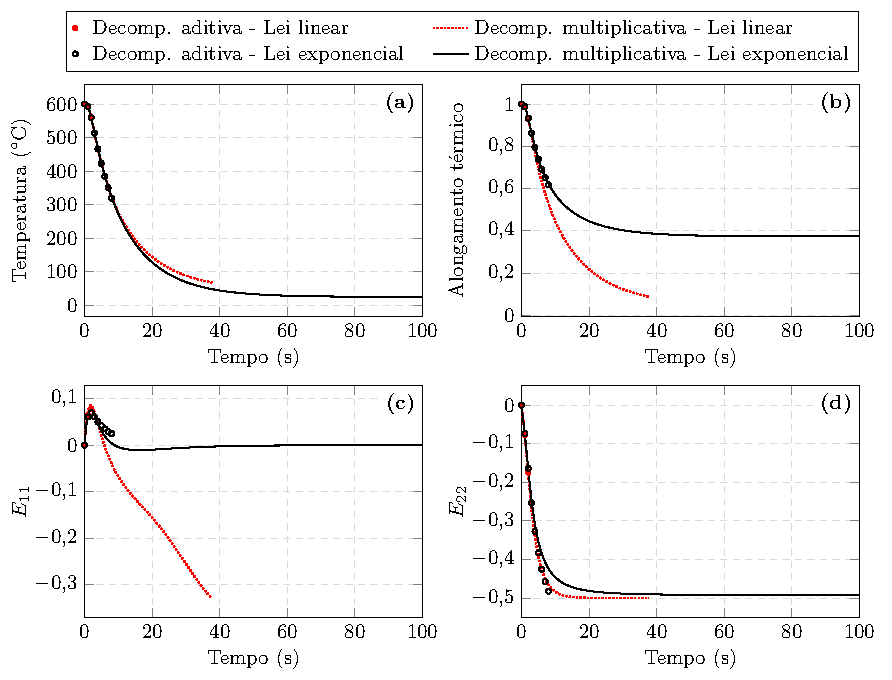
\includegraphics[scale=1.08]{Figuras/ThermoCube3/ThermoCube3Results.pdf}
	%\caption*{\textbf{Fonte:} Elaborado pelo autor}
\end{figure}

Na \autoref{fig:ThermoCube3Stress}, são mostradas as configurações deformadas para diversos passos de tempo do problema, considerando o caso em que é utilizada a decomposição multiplicativa e lei de expansão térmica exponencial. Embora o alongamento térmico mínimo para esse caso seja em torno de $40\%$, conforme indicado na \autoref{fig:ThermoCube3Results}(b), observa-se que a variação de altura é muito menor que $40\%$ devido à contribuição da parcela mecânica de deformação que surge para compensar as restrições no sentido da largura e da profundidade. Ainda na \autoref{fig:ThermoCube3Stress}, são apresentadas no mapa de cores as componentes horizontais da tensão de Cauchy, manifestadas como consequência dessas deformações mecânicas.
\begin{figure}[!htb]
	\centering
	\caption{Tensão $\cauchyind_{11}$ sobre a configuração deformada para o modelo baseado na decomposição multiplicativa e lei exponencial}
	\label{fig:ThermoCube3Stress}
	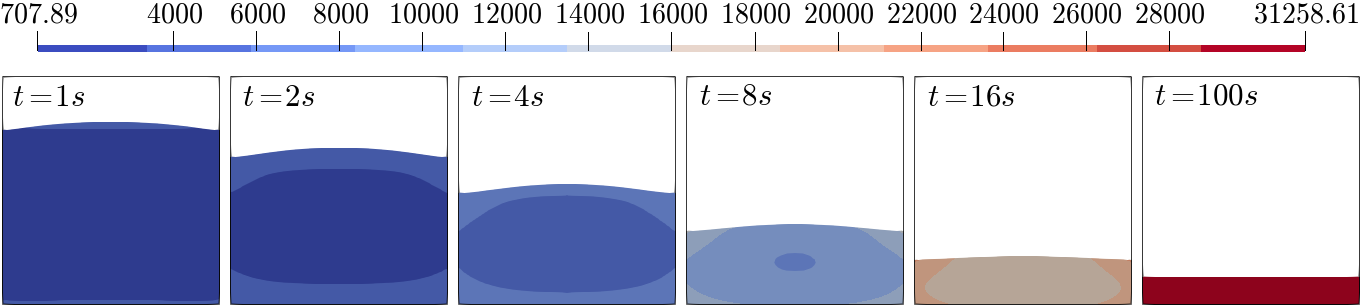
\includegraphics[scale=0.44]{Figuras/ThermoCube3/ThermoCube3Stress.png}
	%\caption*{\textbf{Fonte:} Elaborado pelo autor}
\end{figure}

%\newpage
%\null
%\vfill



\end{document}
	
	
